
\documentclass{sig-alternate-cidr}
%\documentclass{sig-strict}

\usepackage{color}
\usepackage{amsmath}
\usepackage{textcomp}
\usepackage{ifthen}
\usepackage{listings}
\usepackage{fancyvrb}
\usepackage{verbatim}
%\usepackage[noend]{algorithm2e}

%\usepackage[pdftex]{graphicx}
\usepackage{graphicx}
\usepackage{subfig}
\usepackage{calc}
\usepackage{float}
%\usepackage{alltt}

\usepackage{url}

% For generating custom lists (similar to table of contents, list of figures
% etc.)
\usepackage[subfigure]{tocloft}

%\usepackage{hyperref}
%\usepackage[all]{hypcap}
%\usepackage{latexsym}

\usepackage{enumitem}

% Remove spacing around section headings
%\usepackage[compact]{titlesec}
%\titlespacing{\section}{0pt}{*0}{*0}
%\titlespacing{\subsection}{0pt}{*0}{*0}
%\titlespacing{\subsubsection}{0pt}{*0}{*0}

%\usepackage[left=1.05in,right=1.05in,top=1in,bottom=1in]{geometry}

% tweak or comment out the baselinestretch to control how much space for hand-writing comments you get between the lines
%\renewcommand{\baselinestretch}{1.8}

\newcommand{\reminder}[1]{}
%\newcommand{\reminder}[1]{ [[[ {\mbox{$<==$}} #1 ]]] }
%\newcommand{\yoav}[1]{\reminder{#1}}
%\newcommand{\reminder}[1]{
%    \par
%    \colorbox[rgb]{0.8,0.8,0.8}{
%        \parbox{\linewidth}{
%            #1
%        }}}
%\renewcommand{\reminder}[1]{}

\newcommand{\eat}[1]{}

\newtheorem{defin}{Definition}[section]
\newtheorem{ex}{EXAMPLE}[section]
%\newtheorem{lemm}{Lemma}[section]
%\newtheorem{thm}{Theorem}[section]
\newenvironment{example}{\begin{ex} \nopagebreak
  \begin{rm}}{\end{rm} $\Box$ \end{ex}}
\newcommand{\exampleverbatim}[1]{\noindent\normalfont{\texttt{#1}}}
%\newenvironment{definition}[1]{\begin{defin}\begin{rm}({\bf
%    #1})}{{\hfill$\Box$}\end{rm}\end{defin}}
%\newenvironment{lemma}{\begin{lemm}}{{\hfill$\Box$}\end{lemm}}
%\newenvironment{theorem}{\begin{thm} \nopagebreak}{{\hfill$\Box$}\end{thm}}


% Commands for writing syntax
\newcommand{\gn}[1]{{\bf #1}}       % (N)on-terminal
\newcommand{\gt}[1]{{\tt #1}}       % (T)erminal
\newcommand{\gs}[1]{{\it #1}}       % (S)pecial construct

% Verbatim environment for SQL snippets
\DefineVerbatimEnvironment% 
{sql}{Verbatim}{frame=single,numbers=left,fontsize=\scriptsize}

% HACK: Bypass ACM's definition of paragraph as a subsubsection
%\renewcommand{\paragraph}[1]{{\noindent {\bf #1}}}

% Compress whitespace around itemize and enumerate
%\setitemize{topsep=.0em,parsep=0pt,partopsep=0pt,labelsep=0.2em,itemsep=0pt,leftmargin=0.5em}
%\setenumerate{topsep=.0em,parsep=0pt,partopsep=0pt,labelsep=0.2em,itemsep=0pt,leftmargin=0.5em}

% Remove paragraph indentation
%\setlength{\parindent}{0pt}

% Remove paragraph spacing
%\setlength{\parskip}{0pt}
%\setlength{\parsep}{0pt}
%\setlength{\headsep}{0pt}
%\setlength{\topskip}{0pt}
%\setlength{\topmargin}{0pt}
%\setlength{\topsep}{0pt}
%\setlength{\partopsep}{0pt}

% Decrease the line spread slightly
%\linespread{0.99}

% Define our own compact enumerate
%\newenvironment{compact_enum}
%{\setlength{\leftmargini}{1em}
%\begin{enumerate}
%  \setlength{\labelsep}{.3em} 
%  \setlength{\itemsep}{.4em}
%  \setlength{\parskip}{0pt}
%  \setlength{\parsep}{0pt}}
%{\end{enumerate}}

% Define our own compact itemize
%\newenvironment{compact_item}
%{\setlength{\leftmargini}{1em}
%\begin{itemize}
%  \setlength{\labelsep}{.3em} 
%  \setlength{\itemsep}{.4em}
%  \setlength{\parskip}{0pt}
%  \setlength{\parsep}{0pt}}
%{\end{itemize}}

%\addtolength{\topmargin}{-8mm}
%\addtolength{\topskip}{-1mm}

%\DefineVerbatimEnvironment%
%{tree}{Verbatim}{frame=single,fontsize=\scriptsize}

%\DefineVerbatimEnvironment%
%{treeNumber}{Verbatim}{frame=single,numbers=left,fontsize=\scriptsize}

% Project Name
\newcommand{\projName}{{Plato}}

\begin{document}
%\title{\projName: A Model-based DBMS for the Efficient Management of Spatiotemporal Sensor Data
\title{Combining Databases and Signal Processing in Plato
\titlenote{This work was partially supported by NSF awards IIS-1447943 and IIS-1237174.}
}

\author{Yannis Katsis \hspace{1cm} Yoav Freund \hspace{1cm} Yannis Papakonstantinou\\
{\small ikatsis@cs.ucsd.edu \hspace{1cm} yfreund@ucsd.edu \hspace{2cm} yannis@cs.ucsd.edu \hspace*{1cm}}\\\\
\affaddr{CSE Department, UC San Diego}\\
}

\maketitle

%\renewcommand{\rmdefault}{phv} % Arial
%\renewcommand{\sfdefault}{phv} % Arial

\begin{abstract}
Sensors generate large amounts of spatiotemporal data that have to be stored and analyzed. However, spatiotemporal data still lack the equivalent of a DBMS that would allow their declarative analysis. We argue that the reason for this is that DBMSs have been built with the assumption that the stored data are the ground truth. This is not the case with sensor measurements, which are merely incomplete and inaccurate samples of the ground truth. Based on this observation, we present \emph{Plato}; an extensible DBMS for spatiotemporal sensor data that leverages signal processing algorithms to infer from the measurements the underlying ground truth in the form of statistical models. These models are then used to answer queries over the data. By operating on the model instead of the raw data, Plato achieves significant data compression and corresponding query processing speedup. Moreover, by employing models that separate the signal from the noise, Plato produces query results of higher quality than even the original measurements.

%Analysis of spatiotemporal sensor data is crucial for a large number of companies, including electricity, fitness tracking, and environmental monitoring companies. Database Management Systems (DBMSs) have long facilitated easy and declarative analysis of enterprise data. However, they cannot directly applied to spatiotemporal sensor data. We argue that the reason of such a discrepancy is that, in contrast to enterprise data, sensor measurements are not the ground truth but instead incomplete and inaccurate samples of the measured phenomena and present \projName; an extensible DBMS for spatiotemporal data. \projName\ enables declarative querying of sensor data by operating not on the sensor measurements but on the underlying ground truth, which can be represented by a statistical model (which \projName\ can automatically infer through well-known signal processing techniques). By operating on the model, \projName\ achieves significant compression of the underlying data and corresponding query processing speedup.
\reminder{Mention accuracy improvements by separating the signal from the noise.} 
\end{abstract}
\section{Introduction}
\label{sec:introduction}

\reminder{TOO GENERIC, DELETED: With the downward trend in hardware manufacturing costs, recent years saw a significant increase in the number of sensors embedded in devices and structures. From consumer devices, such as cars, smartphones and fitness trackers - to name just a few - to infrastructure, such as road, electrical, computer and weather networks, most man-made products contain an entire array of sensors}
Sensors generate ever increasing amounts of spatiotemporal data that have to be stored and analyzed. However, analysis of spatiotemporal sensor data is a labor-intensive process. In simple cases, the analyst copies (a subset of) the sensor measurements out of the data store to custom software (typically statistical signal processing algorithms),  computes an underlying real world model, utilizes the model in various types of analyses, such as predictions, correlations and outlier detection and copies the results back into the database. In such cases, the database is utilized just as a store. In more complex cases, where the sensor analysis is combined with the context provided by the conventional alphanumeric data of the database, the analyst-specified processing pipeline is effectively a manually provided query plan. 
\reminder{IMO THE WEATHER EXAMPLE IS TOO DANGEROUS BECAUSE ITS MODEL IS TOO APPLICATION-SPECIFIC, THEREFORE PLATFORM DEFYING. For instance, in the case of weather data, custom software uses the measurements taken by weather stations to infer a weather model that predicts the weather conditions in any given location. This model is then used as input to other algorithms performing different types of analyses, such as predictions, correlations etc.
}\reminder{Agreed. I have also removed the discussion on very domain specific models that we used to have in the description of the learning algorithms (Section \ref{sec:models}).}

 By employing a hardcoded processing pipeline for each different analysis case, the state of the art in sensor data processing thus misses all the productivity and performance-enhancing features introduced by Database Management Systems (DBMSs), such as {\em declarative querying}, {\em automatic query optimization} and {\em independence of the physical layer} (specifying how data are stored and queried) {\em from the logical layer} (describing the view of the data to the analyst).

Though it is clear that a merger of signal processing and databases would be beneficial, conventional DBMSs cannot in their current form accomodate spatiotemporal signal analysis. The reason is a key difference in the founding assumptions of databases and signal processing. In contrast to conventional data found in databases, which have a one-to-one mapping to real world objects, the signal processing community assumes that the data are mere {\em measurements} (samples) of the corresponding physical reality.
As such, sensor data are by definition (a) inaccurate, containing apart from the signal corresponding to the physical quantity measured also a noise component which is the result of random influences on the sensor and (b) incomplete, being discrete samples of a continuous signal. It is easy to see that conventional query processing fails under either of these properties. Querying noisy data leads to inaccurate results, without even explaining the extent of the inaccuracy. Similarly, even simple query operations, such as the join of two relations cannot be directly applied to incomplete data, since the two relations being joined may contain measurements that were taken at slightly different times and locations and thus do not align in space and/or time.

\projName\ aims to merge a general declarative DBMS (with all the associated advantages) with the signal processing paradigm, by operating on the underlying ground truth instead of the actual measurements. The ground truth in this case is represented by a {\em model}, which is a continuous function in space and/or time describing the quantity of interest (e.g., temperature, velocity, acceleration, air pollutant concentration etc.). Models have been successfully used in the signal processing community but have not yet been incorporated in DBMSs. The proposed \projName\ DBMS introduces models as first-class citizens. This addition not only enables declarative query processing for spatiotemporal sensor data, but also achieves significant compression compared to the storage of the actual measurements, which in turn leads to improved query processing performance. Lastly, using models that separate the signal from the noise leads also to improved accuracy of the query results. %compared to analyses operating directly on the sensor measurements.

In short, \projName\ proves the value of operating on the reality (as described by the models) rather than on its projection (as given by the raw measurements). This separation between the actual reality and the perceived reality is also the reason for the system's name, in an allusion to Plato's Cave allegory\footnote{In Plato's Cave, a few prisoners are bound, since birth, to look at a wall where shadows of real world's objects appear. The prisoners perceive only the 2-dimensional world of the shadows and miss the deeper insights that a comprehension of the full 3-dimensional reality would offer them.
%Similarly, the sensor measurements that appear in a database are the mere projection of the real world. The insight in the world is captured by physical models (i.e., models that capture the world's physics).
}.
%
Plato proposes the following novelties:

\begin{itemize}
\item A DBMS architecture for spatiotemporal sensor data, containing a novel infrastructure for the definition of models through reusable learning algorithm modules. The models involve a probabilistic aspect that draws from the foundations of signal processing.
\item Two query languages - ModelQL and InfinityQL - for declaratively querying models. Each language is suited to analysts of different backgrounds, exposing the models either as black boxes (best suited to statisticians and users of systems such as R) or as infinite relational tables (a good fit for SQL programmers).
\item A novel hierarchical data store for models, in which the components of a model are stored in a compressed form in order of decreasing importance. This enables:
\item A novel query processing algorithm operating directly on the models that brings significant gains in performance and accuracy compared to a naive solution operating  on the measurements. The query processing algorithm leverages the hierarchical data store to further cut down query processing time by only utilizing the components of the model required to reach the confidence guarantees required by the user.
\item Guidelines for inferring \emph{reduced-noise} models; i.e., models that separate the noise from the signal and thus improve on the quality of the original measurements.

\reminder{Is guidelines the right word to use in this context?}
\end{itemize}







\section{Related Work}

\reminder{Add forward reference to probabilistic DB discussion}

\eat{
\textbf{Prior work from signal processing and machine learning.}
Work on adaptive signal processing starts in the 50's with the
the Wiener filter, followed by the Kalman filter and the Widrow-Hoff
algorithm~\cite{adaptive_signal_processing}. Enormous progress has
been made since that time and adaptive signal processing is now
textbook material~\cite{dsp,adaptive_filter_theory}. Closely related
is data compression theory and practice~\cite{DBLP:books/mk/Sayood12}.
Recent work of the database field in this area is summarized in \cite{DBS-004}.

The last decade has seen the rapid development in the area of online
learning. This is a subarea of machine learning that is based on ideas
from adaptive signal processing and has made interesting and fruitful
connection to information theory and game theory. PI-Freund is active
in this area of research~\cite{prediction_learning_models}.
}

\textbf{Models as tools for compression.} Statistical models, primarily histograms and wavelets, have been widely used for compression in the database literature (see survey \cite{DBS-004}). However, in contrast to \projName, these works assume the contents of the database to be the ground truth, rather than noisy and incomplete measurements thereof. Thus the query answering algorithms lack a probabilistic aspect. Furthermore, most works do not support arbitrary queries, being instead tuned to specific query patterns  (e.g.,  approximate query result size through the use of histograms).\\

\textbf{Model-based data infrastructure.}
The idea of using models as part of a general DBMS was first presented in the context of MauveDB \cite{mauvedb-grid, mauvedb-cidr, mauvedb-vldb}. \projName\ extends these ideas in several important directions: First, MauveDB argues that models need to be discretized in the coordinates' grid, before they can be queried. In this work we show that a fully virtual approach, where the model is perceived as a function over the infinite spatiotemporal domain, is both easier for the data analyst and more opportune for the query optimizer. For instance, consider two temporal models represented by their Fourier transform and a query asking for their correlation. It is most efficient to compute this query directly on the frequency domain rather than bring it back to the time domain. Second, while MauveDB showcases some of the challenges that arise in model-based systems and presents solutions for specific models, it does not contain a general framework that would allow one to plug in arbitrary models (which is one of the main goals of Plato). 
Lastly, other works studied particular point problems related to the use of models to represent sensor data, such as comparing compression ratios or designing indices useful for models \cite{aberer-cloud, aberer-compression}. However, they did not present a general extensible model-based database platform.\\

%Apart from MauveDB, several works studied particular point problems related to the use of models to represent sensor data, such as comparing existing models in terms of compression or designing indices that would be useful for such models \cite{aberer-cloud, aberer-compression}. However, neither of these works described a general extensible database platform that can accomodate and offer extensive query capabilities over a variety of models.

\textbf{Efficient query processing on models.} The idea of evaluating queries directly on the representation of a model without discretizing them first, was presented in the context of FunctionDB \cite{functiondb}. The work showed that for a broad class of polynomial functions, faster processing is achieved by evaluating queries directly on the algebraic representation of the functions. Plato's goal is to provide the platform infrastructure that enables such optimizations for broader classes of statistical models.\\

\textbf{Statistical functions inside DBMSs.} Finally, libraries such as MADLib \cite{madlib} allow statistical functions to be evaluated inside a DBMS. While this solves the problem of moving the data out of the database for processing, it couples model creation with query processing, thus not allowing the use of functions to generate models that are hidden from the analyst and used by the system to process arbitrary queries.

%\textbf{Models as tools for compression.} The database community has extensively researched compression, primarily using histograms and wavelets (see survey \cite{DBS-004}). As is typical in database works, the contents of the database are assumed to be the ground truth, rather than noisy and incomplete measurements of the ground truth. Respectively the query answering algorithms lack a probabilistic aspect. Furthermore, the approximate query processing works have been tuned to few query patterns. E.g., a notable success is the use of histograms in query cost estimators that approximate the expected size of query results. However, there is no query processor architecture work on how to gracefully retreat to reconstruction, when computation directly on the compression is not possible.

\reminder{Add work on (a) signal alignment and (b) sensor networks.}

\section{Why Models?}
\label{sec:model-abstract}

A central idea behind \projName\ is to distinguish between the {\em
  state of the real world}, {\em raw sensory data} and a {\em model of
  the world}. For example, consider the mental process that takes
place when a bird watcher is tracking a goose (see
Figure~\ref{fig:trackingGeese}). In this case the state of the real
world includes the location and orientation of the goose relative to
the bird watcher, the physical appearnce of the bird, and the state of
the flapping of the wings. The sensory information is the light field
as is captured by the eyes of the bird watcher and transmitted to the
brain. Finally, the {\em mental model} is a representation of the real
world as it is preceived in the birdwatchers mind.

\begin{figure}[t]
\center
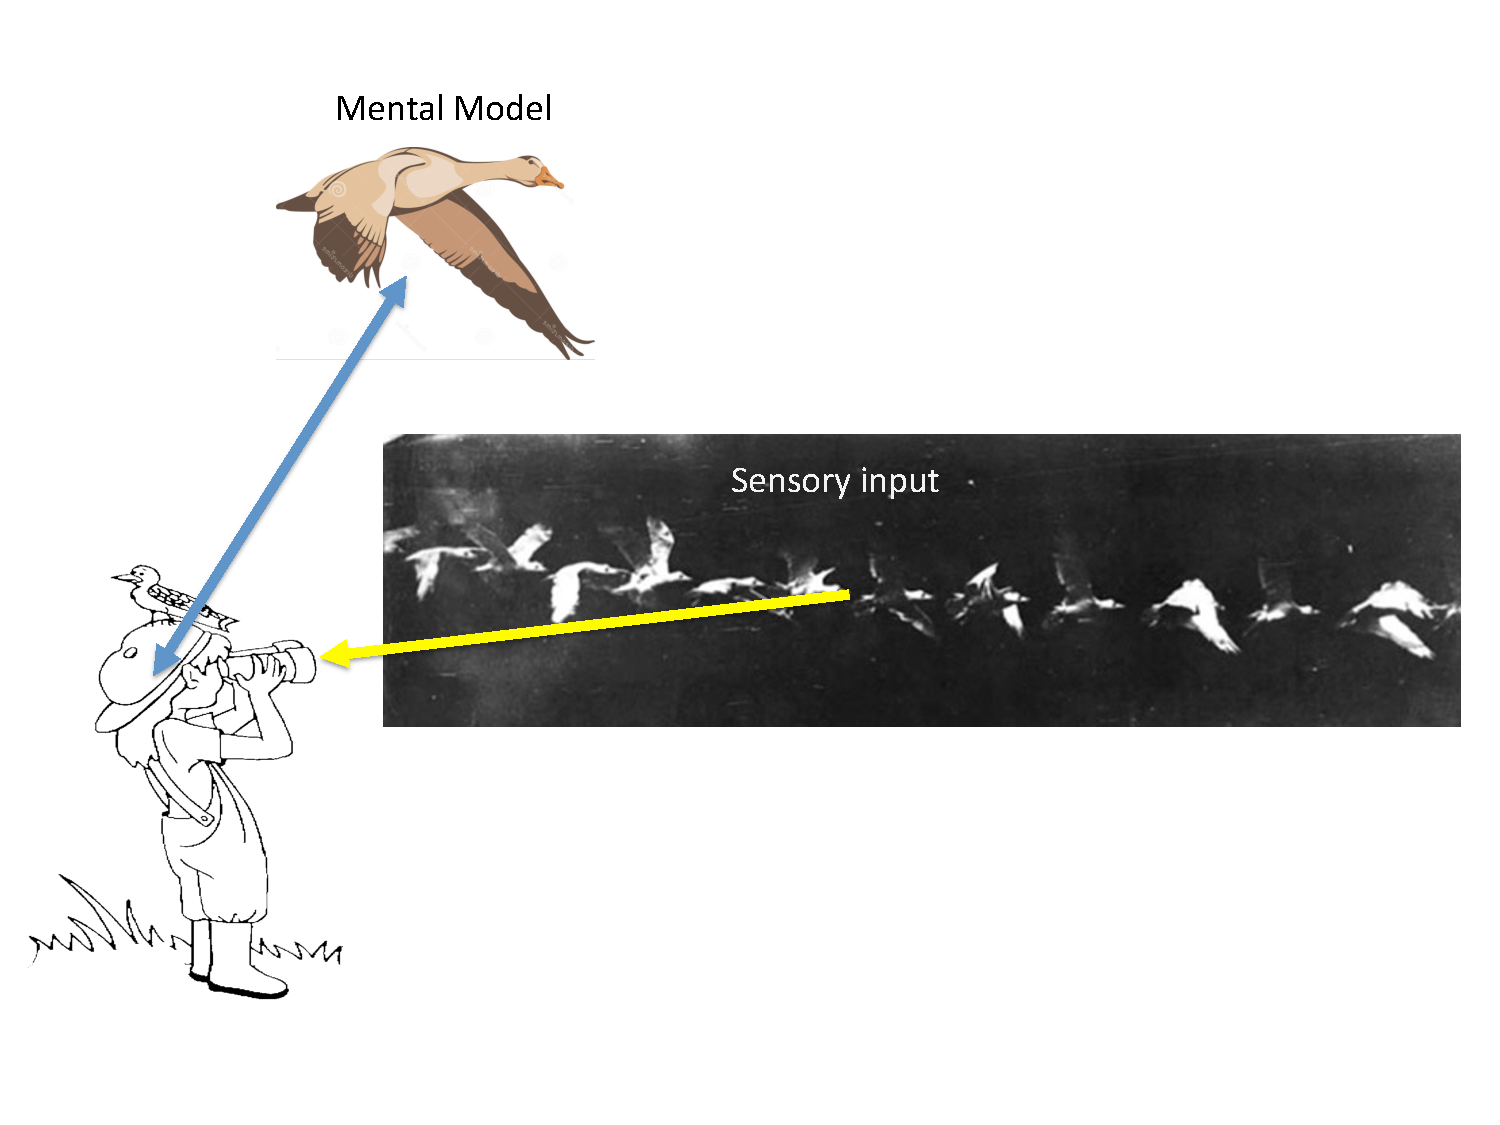
\includegraphics[width=\columnwidth]{TrackingGeese.pdf}
\caption{Bird Tracking Example}
\label{fig:trackingGeese}
\vspace{-0.4cm}
\end{figure}

\emph{The insufficieny of sensory data:} Note that the sensory
information is neither neccessary nor sufficient for tracking the
bird. It is not neccessary because objects other than the bird are
irrelevant to the task. It is not sufficient because poor focus,
glare, obstruction and other sources of {\em noise} and {\em
  distortion} might make it impossible to locate the bird in any single
frame.

\emph{Data integration using a model:} The brain transforms this
imperfect information into pan and tilt commands to the head and eyes
of the observer so as to keep the bird in the center of the field of
view. To do so the brain uses a {\em model} of the bird in flight. In
this simple example the model represents the {\em appearance} of the
bird in terms of shapes and colorsthe {\em movement} of the bird in
space. If this is an experienced bird watcher, the model is highly
detailed and specific and is {\em adapted} to the particulars of the
task.

\emph{Parameters and state:} A typical model consist of two parts:
fixed (or slowly varying) {\em parameters} and a rapidly varying {\em
  state}. In the bird tracking example the parameters might include
the appearance of the bird from different angles and at different
stages of flapping the wings. It contains also a characterization of
the range of speeds and altitudes at which the bird typically flies
and of typical changes in the flight direction.  The {\em state} in
the bird tracking example might include of the pan and tilt angles,
the change rates of these angles, the direction from which the bird is
viewed and the phase of the wing flap cycle.

\emph{Correspondance:} A model is a representation of {\em real world
  system}. If the model is good, then there is a one to one
correspondance between the parameters of the model and the
characteristics of the physical system and between the state of the
model and the state of the system. A main goal of \projName\ is to
construct models whose state corresponds to the state of the real world.

\emph{Learning, tracking and loss functions} the parameters and the
state of the model are adjusted according to the sensory data. We call
the adaptation of the parameters ``learning'' and the adjustment of
the state ``tracking''. The goal of both learning and tracking is to
minimize a {\em loss function}. The loss function takes as input
sensory data and a model and outputs a non-negative number. If the
loss (or the average loss) is low we say that the model {\em conforms}
with the data.


\emph{Models and compression} One of the ways in which a conforming
model can be used is to {\em compress} the data. Models that conform
to the data can usually be transformed into {\em predictive} models
which predict future values based on past values. Compression is
achieved by encoding the data as a sequence of differences between the
prediction and the measurements. If the predictions are accurate, the
number of bits required to store the differences is much smaller than
the number of bits required to store the raw data. Compression comes
in two flavors: {\em lossless compression} (such as the Lempel-Ziv method)
allows perfect reconstruction of the original signal, while {\em lossy
  compression} (such as DPCM, MP3 and JPEG2000) allows only
approximate reconstriction. On the other hand, the compression ratio
achieved by lossy compression is typically much higher.

\emph{Compression Bias} Lossy compression is not free. Lossy
compression using a poorly chosen model which does not represent the
measured reality can create artifacts in the reconstructed data. In
some cases the artifacts can mask important state data.

\emph{Noise reduction} If the model is well chosen and it's parameters
and state corrspond to those of the measured reality, the
reconstructed data can be a {\em better } representation of the state
of reality than the raw signal. That is related to the fact that
common types of noise, in particular {\em additive white noise} have high
information content (entropy) and are impossible to compress. Removing
the white noise component results in a win-win situation where the
compressed signal is highly comressed and the reconstructed signal is
a better representation of the state of reality than the raw signal.

\subsection{Notation}

We use the following notation to represent the above mentioned
concepts.

\newcommand{\cM}{{\cal M}}
\newcommand{\cSM}{{\cal SM}}

\begin{itemize}

\item Denote the spatiotemporal space by $X$ and call a particular
  element $x \in X$ a point. (Typically $a$ defines both location and time).

\item A measurement is a pair $(x,y)$ where $x$ is the location (in
  space and time) in which the measurement was taken and $y \in Y$ is the
  quantity measured. We will refer to $Y$ as the outcome space. The
  outcome space can be a scalar (for example, a temperature
  measurement), a vector (for example, an image) or a (potentially
  infinite) sequence of measurements:$y_1,y_2,y_3,\ldots$.

\item A stateless model $\cM$ is a is a function that maps from $X$ to a
  prediction space $\Lambda$.  

\item The outcome space $Y$ and the prediction space are linked
  through a Loss function $\gamma:\Lambda \times Y \to R^+$ where
  $R^+$ is the set of non-negative reals. A good prediction is one
  which induces a small loss. Below we describe a few popular
  outcome/prediction pairs.

\item A model with state (also called a ``filter'') which we denote by
  $\cSM$, consists of a state $s \in S$ and two
  functions $A: S \times Y \to S$ and $O: S \to \Lambda$. The
  model assumes that the time is descrete and sequential.
  The initial state $s_0$ is assumed to be of no long term importance
  (i.e. the markov model defined by the model plus nature is rapidly
  mixing). The model takes as input a sequence of inputs
  $y_1,y_2,\ldots$ and performs the following two steps for $t=1,2,3,\ldots$:
  \begin{enumerate}
    \item Update state (Track): $s_t = A(s_{t-1},y_t)$
    \item Produce prediction: $\lambda_t=O(s_t)$
  \end{enumerate}

\item A learning algorithm takes as input a {\em training set}, which
  is a set of $m$ measurements$\{(x_1,y_1),\ldots,(x_m,y_m)\}$ and
  outputs a model $\cM$ or $\cSM$ which  has low loss with respect to
  a given loss function $\gamma$.
\end{itemize}

\subsection{Queries}

\subsubsection{Simple Queries}

A point query specifies a location $x \in X$ and asks the model to
make a prediction on $x$, where the prediction an element in the
outcome space, i.e. $y \in Y$. Typical loss functions for this case
are $(\cM(x)-y)^2$ or $|\cM(x)-y|$.

A range query specifies a location $x$ and asks the model to predict a
range $[a,b]$ (or, more generally, a set) that contains the outcome
$y$. The loss function that is associated with this case is the binary
function that is $0$ in the range $[a,b]$ and $1$ outside of this
range.

\subsubsection{Statistical Guarantees for simple queries}

Statistical guarantees are stated about a model as a whole, not about
the prediction on specific locations. There are three major types of
guarantees:

\begin{itemize}
\item {\bf Worst-case or max-norm guarantees} These are guarantees of
  the form: with probability 1-over the random choice of the training
  set the learning algorithm generates a model $\cM$ such that: For
  any measurement $(x,y)$ the outcome y is within predicted range
  $[a(x),b(x)]=m(x)$ Note that in this case evaluating using a model
  that predicts a single number and a loss function is a special case
  of the range model.
\item{\bf Average-case guarantees} In this case the test locations are
  chosen using the same distribution as that of the training set. The
  guarantee takes the form: with probability 1-over the random choice
  of the training set the learning algorithm generates a model m such
  that: A test example (test measurement) $(x,y)$ is chosen
  independently at random according to the same distribution that
  generated the training set. Our guarantee is on the expected value
  of the loss function $E(x,y)m(x),y$ more precisely, we say that with
  probability 1-over the random choice of the training set the
  learning algorithm generates a model m such that: $E_{(x,y)}[\gamma(m(x),y)]$ In
  this case a model that predict with a range can be given an
  average-case guarantee, using the range-based loss function.

\item{\bf Statistical significance} This guarantee is the weakest, and
  therefore the easiest to prove. In this case we compare the model we
  generated with a model that was agreed upon a-priori. That
  agreed-upon model is the {\em Null Hypothesis}. The null hypothesis
  defines a distribution over the test measurements. The model
  generated by the learning algorithm is called the {\em Alternative
  Hypothesis}. The type of guarantee given in this case is that the
  probability of the training set according to the Null hypothesis is
  much smaller than the probability of the set according to the
  Alternative Hypothesis. Specifically, the P-value by which we can
  reject the null hypothesis (and adopt the alternative) is the
  probability of the training set (and any set ``more extreme than it'')
  according to the null.

\end{itemize}

\iffalse
the observation that sensor data can be stored
and processed much more efficiently if one operates not on the actual
measurements but on a model of the underlying reality that can be
built from the former. But what is a model? In statistics a model is a
statement about reality. This statement could be of any form. For
instance, a model could be a fundamental law (e.g., Newton's law of
acceleration, stating that the force vector $\vec{F}$ can be inferred
from the acceleration vector $\vec{a}$ and the mass $m$ through the
formula $\vec{F}=m \vec{a}$) or a statement about a physical quantity
in space and/or time in the past (e.g., the temperature at the
entrance of the compute science department at UC San Diego on August
19, 2014 at 9am was between 68 and 70 degrees). But it could also be a
predictive claim about the future (e.g., the average temperature of
the earth will increase by at least 5 degrees between 2014 and 2050),
or a theory (e.g., a medical theory stating that the statins decrease
the chance of a heart attack by more than 20\%).
\fi

\subsection{Model queries}
Higher order queries regard the models, rather than the raw
data. There can be queries regarding the state of the model (what are
the pan/tilt angles that would point towards the bird) or about the
parameters of the model (How does this type of bird look when seen
from a particular angle?).

To be continued.

\section{Older ``Models'' section} 

\projName\ is based on the observation that sensor data can be stored and processed much more efficiently by operating not on the actual measurements but instead on a model of the underlying reality that can be inferred from the measurements. What is a model? In statistics a model is a statement about reality, which could be in general of any form. For instance, a model could be a fundamental law (e.g., Newton's law of acceleration, stating that the force vector $\vec{F}$ can be inferred from the acceleration vector $\vec{a}$ and the mass $m$ through the formula $\vec{F}=m \vec{a}$) or a statement about a physical quantity in space and/or time in the past (e.g., the temperature at the entrance of the computer science department at UC San Diego on August 19, 2014 at 9am was between 68 and 70 degrees). But it could also be a predictive claim about the future (e.g., the average temperature of the earth will increase by at least 5 degrees between 2014 and 2050), or a  theory (e.g., a medical theory stating that the statins decrease the chance of a heart attack by more than 20\%).

Since we are interested in the processing of sensor data with a spatiotemporal component, in this work we restrict our focus to \emph{quantitative spatiotemporal models}; i.e., models that provide the value of a physical quantity for points in space and/or time. An example of a quantitative spatiotemporal model is a function outputting the temperature at the entrance of the computer science department at different points in time. Signal processing has long recognized the value of operating on models inferred from the measurements, instead of operating on the actual measurements themselves.\\

{\bf Advantages of models.} The reasons for preferring models over the raw measurements are multifold: Compared to raw sensor readings, models offer several advantages:
\iffalse
\begin{itemize}
\item \emph{They are functions with possibly infinite domains.} Raw sensor readings are merely discrete samples of an underlying continuous phenomenon (i.e., they provide values of the measured quantity only for a finite number of points in space and/or time). In contrast, models provide also all intermediate values, intuitively ``filling in" the gaps left by the raw measurements in the spatiotemporal dimensions. Having the values of the measured quantity for all points in space and/or time is especially important when joining two spatiotemporal signals on their spatiotemporal component, as otherwise the two signals may not be aligned. For instance, consider the following two datasets: A dataset containing air quality measurements taken at various locations and times at UC San Diego and another dataset containing GPS readings representing the location of a person walking around campus. If we want to compute the quality of the air the particular person was breathing during the walk, we would have to join these two datasets. However a conventional relational join on the space/time attributes of the two datasets will most probably yield the empty result, as the person may have never been at the exact time and location the air quality measurements were taken. Abstracting out each of these two sets of measurements through a corresponding model solves this problem and facilitates the join, as each model will provide the values for every point in space and time.
\item \emph{They offer predictive abilities.} In addition to providing values for points in space and/or time between those for which there exist raw measurements, models may also provide predictions for future points in time, thus allowing users to ask predictive queries. For instance, an air quality model may support queries about the expected air quality tomorrow. Intuitively, the predictive nature of the models stems from the fact that instead of focusing on the actual measurements, models instead capture the (typically recurring) pattern of the underlying phenomenon.
\item \emph{They improve accuracy.} By capturing the pattern of the underlying phenomenon, models may also be able to separate the noise (inevitably introduced in raw measurements due to the limited accuracy of sensors and other random factors) from the actual signal, leading to values that are more representative of the actual reality than the sensor measurements themselves. We will discuss in Section \ref{sec:compression} how models may separate the noise from the signal returning values that are more accurate than the original raw measurements.
\item \emph{They capture uncertainty information.} Even if a model cannot completely separate the noise from the signal, it can explicitly capture the uncertainty that exists in the reported value for the measured quantity. This uncertain information is then leveraged by the query processing algorithms to generate query answers that themselves capture uncertainty. We will outline in Section \ref{sec:probabilistic-models} different ways in which a model can capture uncertainty and describe their relationship to existing works in uncertain and probabilistic databases.
\item \emph{They can be represented compactly.} Finally, models can be most of the time represented more compactly than raw measurements. This not only reduces the storage requirements for the - typically large - sensor datasets, but leads in many cases also to more efficient query execution, as queries can often be evaluated directly on the compressed model representation, as we will discuss in Section \ref{sec:query-processing}.
\end{itemize}

We next describe how \projName\ incorporates models and their associated advantages into a relational DBMS.

\fi
	
% model class
% light integration of models with relational data Vs deep integration
% UDFs: is it like a UDF or is it a UDF? Are tables with UDFs allowed to have code + data.

\section{Plato: A model-aware DBMS}
\label{sec:architecture}

\begin{figure}
\center
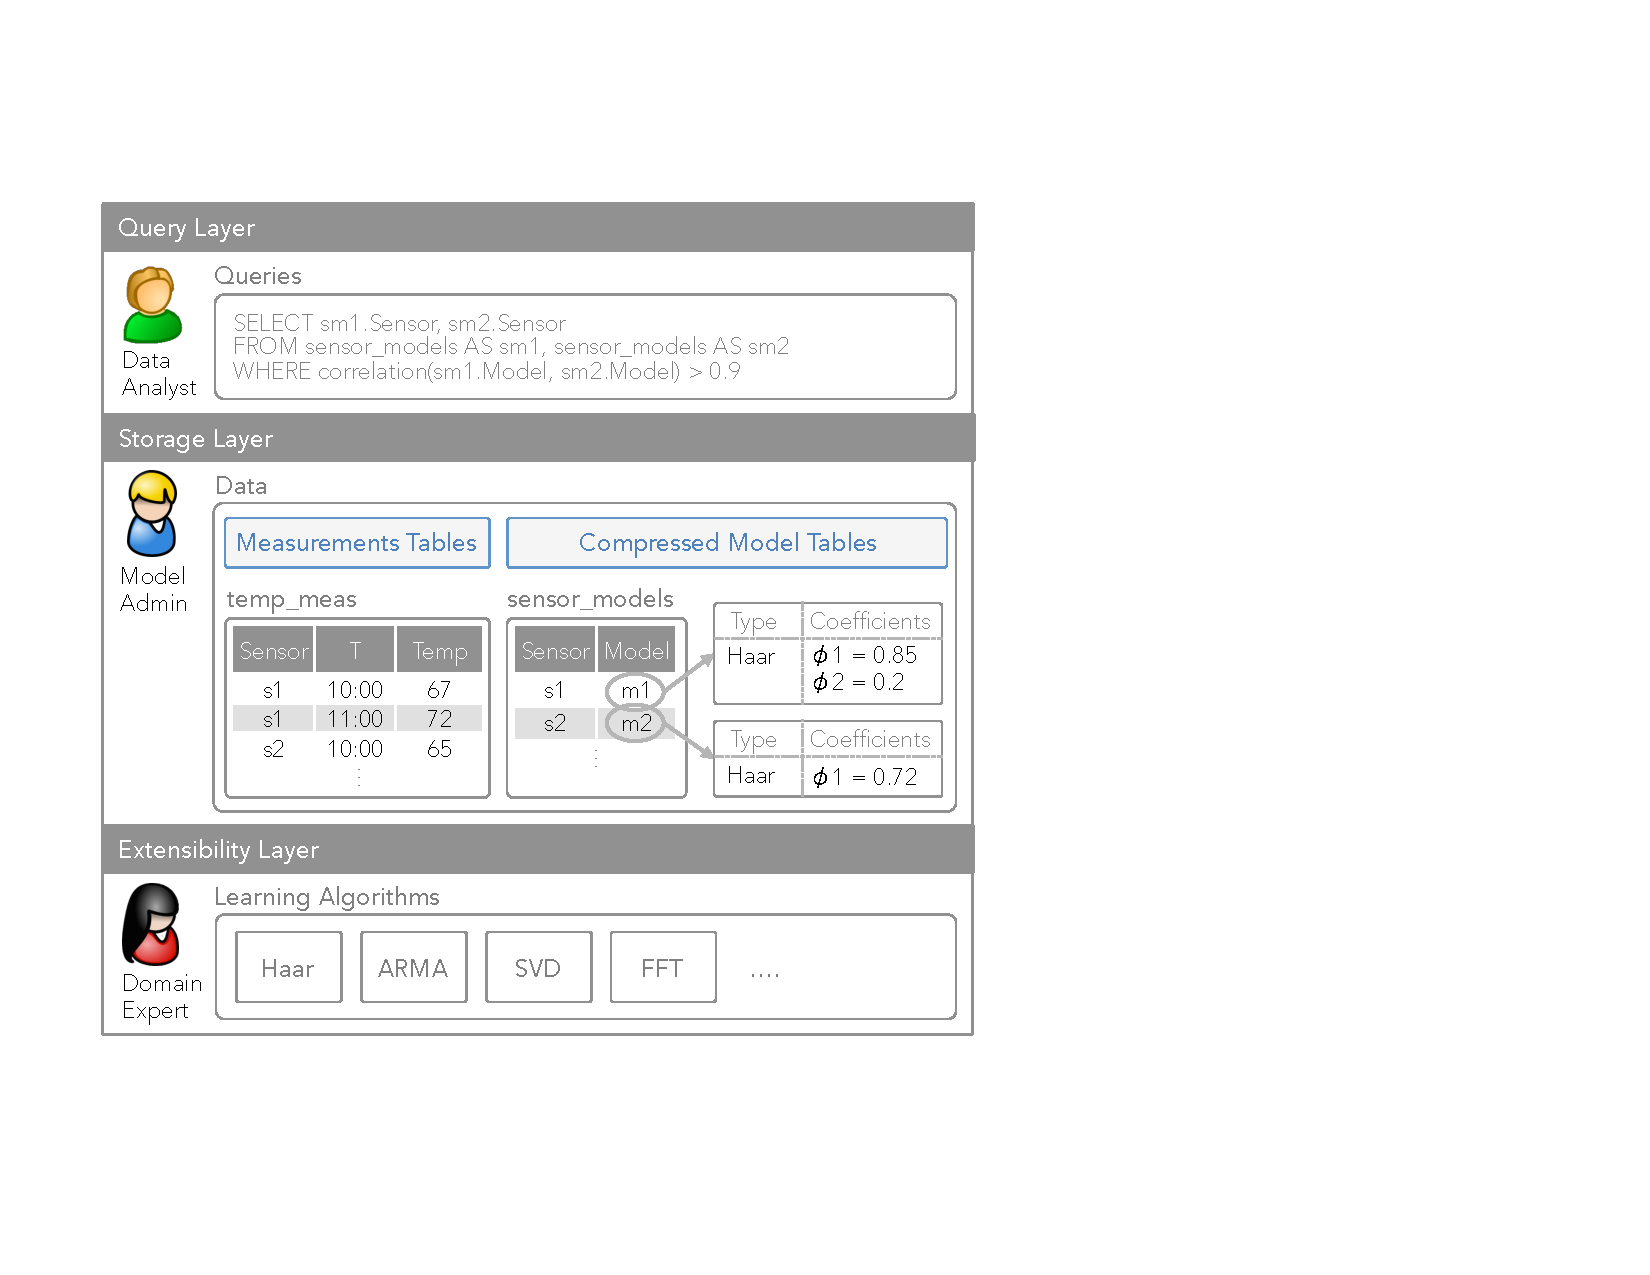
\includegraphics[width=\columnwidth]{fig-architecture2.pdf}
\caption{\projName's Architecture}
\label{fig:basic-architecture}
\vspace{-0.4cm}
\end{figure}

\projName\ enables declarative and efficient querying of spatiotemporal data through the architecture shown in Figure~\ref{fig:basic-architecture}. The system interacts with three different types of users: \emph{Domain experts} with knowledge of statistics and signal processing write learning algorithms, which given raw data create a model over the data using a particular statistical technique (e.g., Wavelets, Fast Fourier Transform, etc).
%These learning algorithms can be either tailored to a particular use case (e.g., an algorithm generating a model for weather data), or be general algorithms that work for entire classes of use cases (e.g., an FFT algorithm).
Out of these registered learning algorithms, \emph{model administrators} with knowledge of a particular dataset, choose a learning algorithm and instantiate its parameters to create a good model for the particular data set. Finally, \emph{data analysts} query the generated models using a declarative query language. We next present the components of \projName\ enabling this workflow. As our running example, we will be using temperature data collected from sensors placed in offices across UC San Diego's campus, in the context of the Energy Dashboard project\footnote{http://energy.ucsd.edu}.

\subsection{Preliminaries}
\label{sec:prelims}

In this work we consider sensor measurements with a spatial and/or temporal component. Let  $D_{xyzt}$ be the spatiotemporal domain that includes the 3D space and the time dimension and $D_{desc}$ a subspace thereof. The subscript $desc$ in $D_{desc}$ describes the dimensions included in the subspace together with any range restrictions. For instance, $D_{xy: (x-x_0)^2+(y-y_0)^2 = r^2}$ contains all 2D points within a circle centered at $(x_0, y_0)$ with radius $r$. Finally, let $X$, $Y$, $Z$, and $T$ be the relational attributes corresponding to the three spatial and the temporal component, respectively.\\

{\bf Storing raw measurements.} We consider sensor measurements that are stored together with their coordinates in conventional relational tables, which we refer to as {\em measurements tables}. A measurements table contains among others a subset of the spatiotemporal attributes $X$, $Y$, $Z$, and $T$ together with a numerical attributes containing values of one or more measured quantities.

\begin{example}
For instance, table \texttt{temp\_meas(Sensor, T, Temp)} of Figure~\ref{fig:basic-architecture} is a measurements table containing tuples of the form $(s, t, m)$, denoting that temperature sensor $s$ provided the temperature measurement $m$ at time $t$.
\end{example}

\subsection{Deterministic Models}
\label{sec:deterministic-models}

To enable declarative querying of spatiotemporal data, \projName\ allows the creation of models on top of the raw measurements. For now, we focus on deterministic models (i.e., models that do not contain any uncertainty), before showing how the concept of a model can be extended to capture the uncertainty inherent in sensor data. A deterministic model is intuitively a mathematical representation of the world that predicts a quantity of interest (e.g., temperature) at every point of the spatiotemporal domain. Formally:

\begin{defin}
A {\em deterministic model} is a function $f:\mathcal{D}\mapsto \mathbb{R}$ from a spatiotemporal domain $\mathcal{D} \subseteq \mathcal{D}_{xyzt}$ to the set $\mathbb{R}$ of real numbers.~\footnote{Although, for ease of exposition we restrict ourselves to models that return a single numeric value for each point in $\mathcal{D}$, in general a model could return values for more than one numerical attributes, i.e., a model could be a function  $f:\mathcal{D}\mapsto \mathbb{R}^n$, $n \ge 1$.}
\end{defin}
\reminder{Do we want to define the probabilistic models here instead of waiting to define them later?}

\begin{example}
For instance, function $f:\mathcal{D}_{t: 2012 \leq t \leq 2013}$ $\mapsto \mathbb{R}$ is a model for temperature, which given a point in time $t$ between 2012 and 2013 returns a real number corresponding to the \emph{predicted} temperature at time $t$.
\end{example}

{\bf Generating models.} Instead of writing models by hand, the model administrator creates models through {\em learning algorithms}, which take as input the measurements and potentially background knowledge about the real world and return a model fitting those measurements. The signal processing community has proposed a set of learning algorithms that have been shown to be applicable to a wide range of domains \cite{dsp}. These include among others algorithms for learning ARMA (Autoregressive-moving-average) models (which are suitable for representing natural phenomena, such as temperature, where the present value depends on the recent past), SVD (Singular Value Decomposition) models, FFT (Fast Fourier Transform), Haar wavelets etc. \projName\ comes preloaded with several such learning algorithms and can be extended by domain experts with additional algorithms.

%Learning algorithms are designed by domain experts, who have knowledge of the domain and the underlying physical properties of the sensor data. For instance, weather experts can design a weather learning algorithm. Although some of the learning algorithms will be domain specific (such as the weather example above), most will be standard signal processing algorithms that are by now textbook book material and which have been shown to be applicable to a wide range of domains. the machine learning community has suggested several algorithms that are applicable to a wide range of domain. These include among others algorithms for learning ARMA (Autoregressive-moving-average) models (which are suitable for representing natural phenomena, such as temperature, where the present value depends on the recent past), SVD (Singular Value Decomposition) models, FFT (Fast Fourier Transform) etc. To bootstrap the system and facilitate the quick generation of models for many common use cases, \projName\ comes preloaded with several such learning algorithms. 

\reminder{To YP: During our discussion, you mentioned that we can claim that with four classes of algorithms we can claim that we cover most of the use cases. Which are these four classes?}

\begin{defin}
A \emph{learning algorithm} $g$ has the general form $g(R;\bar{p})$, taking as input a measurements table instance $R$ and a (variable-length) tuple $\bar{p}$ of parameter values and returning a model.
\end{defin}

The variability of the length of $\bar{p}$ is crucial to ensure that the learning algorithm can be adapted to different scenarios (e.g., domains of different dimensionality).

\begin{example}
For instance, the learning algorithm\\$haar(R;\langle{\bar{A}_{cont}}; A_{meas}\rangle)$ takes as input a measurements table $R$ together with the set $\bar{A}_{cont}$ of attributes of $R$ that correspond to the spatiotemporal attributes and the attribute $A_{meas}$ of $R$ that corresponds to the measurement attribute of interest and creates a Haar model $f:\mathcal{D}\mapsto\mathbb{R}$, where $\mathcal{D}$ is the subspace of the spatiotemporal domain defined by attributes $\bar{A}_{cont}$.
\end{example}  

{\bf Incorporating models into relational tables.} To enable the seamless combination of models with standard relational data, \projName\ allows models to be used as values in tables. In addition to SQL's data types (e.g., string, integer, etc.), \projName\ also provides a new {\em model data type} that comes with an associated model signature $\mathcal{D}\mapsto \mathbb{R}$. An attribute of such a type is called a {\em model attribute} and accepts as values models conforming to the corresponding  signature. We will refer to a table that contains at least one model attribute as a {\em model table}. Model tables are defined by SQL view definitions that involve {\em learning algorithm} invocations. 

\begin{example}
\label{xmpl:models-and-definitions}
%The following statement creates the model table \texttt{sensor\_models} of Figure \ref{fig:basic-architecture}, containing pairs of sensor ID and ARMA model, describing the predicted temperatures of the corresponding sensor:
%
The following statement creates out of the measurements table \texttt{temp\_meas} the model table \texttt{sensor\_} \texttt{models}, containing sensor IDs and Haar models, describing the predicted temperatures of the corresponding sensors:

\begin{verbatim}
CREATE MATERIALIZED VIEW sensor_models AS 
SELECT Sensor, haar(G; <T; Temp>) AS Model
FROM temp_meas GROUP BY Sensor AS G(T, Temp)
\end{verbatim}

For ease of exposition, we use an extension of SQL that allows the creation of nested tables. In particular, the GROUP BY operator creates for each sensor in the measurements table \texttt{temp\_meas} a nested table $G$ with all measurements for that sensor. This nested table is given as input to the Haar learning algorithm to create the corresponding model.
%The resulting model table \texttt{sensor\_models(Sensor, Model)} contains tuples of the form $(s, f)$, where $s$ is a sensor and $f$ the corresponding temperature ARMA model.
\reminder{To YP: Is there a standard nested relational extension of SQL we could reference?}
\reminder{To YP: We present nested tables in passing (both here and in the InfinityQL definition. Should we make it more prominent by defining our data model to be the nested relational?}
\end{example}

Similarly to conventional views, a model table may be virtual or materialized. In practice, the model administrator is motivated to materialize models (and the respective model tables) in order to benefit from the data compression that models enable, as we will discuss in Section \ref{sec:compression}. This can be achieved by using the MATERIALIZED keyword in the model table definition as shown above.\\

\reminder{Discuss choosing between different models}

%Note, that the administrator has in general to choose in general between multiple model algorithms, which come with different compression levels and corresponding guarantees regarding information preservation. Indeed, a major research issue, discussed in Section~\ref{sec:compression}, is the semiautomation of the choice of model algorithms, which should take into consideration the query/analytics workload.

\reminder{Removed example of modified schema}
\eat{
\begin{example}
In a modification of the running example, the administrator can choose to capture temperature in a single model \texttt{full\_model} that predicts the temperature based on \texttt{x}, \texttt{y} and \texttt{t} and is defined as follows:
\begin{verbatim}
CREATE MATERIALIZED VIEW full_model AS 
haar(SELECT X, Y, T, Temp
FROM temp_meas, temp_sensor WHERE Sensor = ID; X, Y, T; Temp)
\end{verbatim}

The reasons for doing so could be: (a) The individual sensor models may be heavily correlated based on the \texttt{X} and \texttt{Y} sensor coordinates. In such case, a single model can have a much more compact representation than the collection of individual sensor models.
(b) The analytics may need temperature predictions for specific locations, which do not coincide with any individual sensor.
\end{example}
}
%\paragraph{Vector quantities} In the general case, a model's quantity is a vector (rather than a scalar) from the domain $\mathcal{\bar{Q}}$.

\subsection{Probabilistic Models}
\label{sec:probabilistic-models}

For ease of exposition,
models have been defined above as functions returning absolute values. However,
since they are inherently statistical approximations of the underlying
process (as they are based merely on measurements), models should have a
probabilistic component. Adding probabilistic information to a model
can be done in several ways. We next outline three alternatives, explain
their connection to prior works in probabilistic databases and signal
processing, and argue for the one we adopt in \projName. In the
subsequent definitions we assume that the domain of the model is
$\mathcal{D} \subseteq \mathcal{D}_{xyzt}$ and its intended range
(leaving aside the probabilities for a moment) is $\mathbb{R}$.\\

\noindent \emph{Model as a probability distribution over functions.} A
\emph{function-probability} model is a probability distribution over
all functions $f:\mathcal{D} \mapsto \mathbb{R}$. Drawing an analogy
with probabilistic databases, a function-probability model corresponds
to a probabilistic database defined as a probability distribution over
the set of database instances that constitute the set of possible
worlds.%
\footnote{In an even wider interpretation, a propability function characterizes the entire database and allows the expression of dependencies across different tuples and models.}
Although this definition of probabilistic databases is very
general and thus guaranteed to cover any use cases, we are not
aware of any practical system employing it. Similarly, we argue that
function-probability models are merely of theoretical interest.\\

\noindent \emph{Model as a probability distribution over values.} A
\emph{value-probability} model is a function from $\mathcal{D}$ to
probability distributions over $\mathbb{R}$. Continuing our analogy, this
corresponds to probabilistic databases where each tuple has
a set of possible instantiations with associated probabilities that
are independent of those of the other tuples. Since each point in
$\mathcal{D}$ is assigned a probability distribution independently of the
other points, value-probability models are strictly less expressive than
function-probability models. However, value-probability models are
still too general for practical use as they may attach an arbitrary
probability distribution to a point in the domain $\mathcal{D}$.
These probability distributions may be hard to infer from the data,
hard to represent in a compact way and more importantly, they may
contain more information than is really needed to reason about the data.
Indeed, statisticians and practitioners often argue that knowing the exact probability distribution
of the possible values for a point in $\mathcal{D}$ is not of
practical importance. In order to make decisions based on the data, it suffices to
know the range in which a value almost certainly will fall. This leads to
the third definition of probabilistic models, inspired from statistics.\\

%To this end, we introduce a third definition of probabilistic models, which leverages the tried-and-true work of the signal processing community in modeling signals.\\

\noindent \emph{Model as a set of prediction intervals.} A \emph{prediction-interval} model is a function from $\mathcal{D} \times \mathcal{P}$ (where $\mathcal{P}$ the set of allowable p-values) to the set $\mathbb{R}_{interval}$ composed of triples of the form $(v, -\epsilon_1, +\epsilon_2)$, where $v, \epsilon_1, \epsilon_2 \in \mathbb{R}$. The semantics are the following: Let $d$ be a value in the domain $\mathcal{D}$, $p$ a p-value in $\mathcal{P}$ and $(v, -\epsilon_1, +\epsilon_2)$ the interval returned by the model for $(d, p)$. Then, according to our current knowledge, the value corresponding to point $d$ is in the interval $[v -\epsilon_1, v + \epsilon_2]$ with probability at least $1-p$. The p-values are typically chosen from a set of values close to zero (commonly below 10\%). Since the p-value $p$ is close to zero, the probability $1-p$ of the value being in the specified interval is close to one, making this an almost certainly true statement.

The inclusion only of statements that are almost certainly true is a fundamental departure from probabilistic databases, where one is interested in the probability of all possible events, however small that probability might be. Although general probabilistic databases have certainly their place in many scenarios (e.g., they are ideal candidates to store inferences made by bayesian networks), in this work we will adopt this restricted form of probabilities, as it has been proven in statistics to work well for decision support that leads to actionable items.

Note, that in addition to almost certainly true facts (i.e., facts that are true with probability at least $1-p$), a model may also include almost certainly false facts (i.e., facts that are false with probability at least $1-p$). This is essential in order to create a model that is closed under queries involving negation (which could start from a set of almost certainly true facts and infer a set of almost certainly false facts).

The signal-processing community has successfully used a special case of this model, briefly explained below.\\ 

\noindent \emph{Model as a combination of signal and noise.} A
\emph{signal-noise} model is a special case of the \emph{prediction-interval} model, where the intervals $(v, -\epsilon_1, +\epsilon_2)$ for each $(d, p)$ pair in $\mathcal{D} \times \mathcal{P}$ are not given explicitly, but instead described indirectly through two components: (a) the center of the interval (i.e., the value $v$) at any point in $\mathcal{D}$ and (b) a gaussian distribution $N(0,1)$ together with its amplitude at any point in $\mathcal{D}$, which are used to compute the range of the interval (i.e., the values $-\epsilon_1$ and $+\epsilon_2$) at any point in $\mathcal{D}$. The first component represents the \emph{signal}, while the second represents the \emph{noise}. In particular, for a given p-value a signal-noise model is a function $f(i) = s(i) + \alpha(i)
n(i)$, $\forall i \in D$, where $s: \mathcal{D} \mapsto \mathbb{R}$
is a non-probabilistic function representing the signal, $n$ is {\em white noise} (i.e., the well-known gaussian distribution $N(0,1)$  \cite{dsp}) and $\alpha: \mathcal{D} \mapsto \mathbb{R}$ is a function representing the amplitude of the noise at any point in $\mathcal{D}$.
\reminder{Do we want to have a special case of the above definition,
where we use the same probability distribution for all points in
$\mathcal{D}$?} \reminder{In theory yes. But I wrote that we leverage
``signal processing work" and i do not know of such work. I was more
comfortable adding the white noise specialization.
}\\

\projName\ employs the prediction-interval probabilistic model and its signal-noise specialization as their value in capturing real use cases has been successfully proven by
the signal processing community. Moreover, the latter approach allows models that separate the signal from the noise, leading to high quality data,
as we will discuss in Section \ref{sec:compression}.

%models return in reality probability distributions of the quantities, rather than absolute values. Therefore a model is a function $f:\mathcal{D}\mapsto \mathcal{H_{Q}}$, where $\mathcal{H_{Q}}$ is the space of probability distributions over the quantity domain $\mathcal{Q}$. The probability distributions capture the certainty of the predicted values. For example, the model of Example~\ref{xmpl:models-and-definitions} can easily benefit from returning probability distributions of the predicted temperatures. A common way of displaying the probability distribution of a quantity to the end user is through a triple $(p, v, \epsilon)$, denoting that the the quantity's value falls within the interval $[v - \epsilon, v + \epsilon]$ with probability $p$.\\

%\paragraph{Viewing models as infinitely-sized tables} Notice that a model $f:\mathcal{\bar{D}}\mapsto \mathcal{H_{\bar{Q}}}$ can be also perceived as a table $R_f(\bar{D}, \bar{Q}, H)$, where the table has an infinite number of tuples, the coordinates $\bar{D}$ form a key and the attribute $H$ provides the value of the probability distribution at the specific coordinates.
%Correspondingly, the models that are the values of a table's attribute can be perceived as infinite size nested tables.%

%models return in reality probability distributions of the quantities, rather than absolute values. Therefore a model is a function $f:\mathcal{D}\mapsto \mathcal{H_{Q}}$, where $\mathcal{H_{Q}}$ is the space of probability distributions over the quantity domain $\mathcal{Q}$. The probability distributions capture the certainty of the predicted values. For example, the model of Example~\ref{xmpl:models-and-definitions} can easily benefit from returning probability distributions of the predicted temperatures. A common way of displaying the probability distribution of a quantity to the end user is through a triple $(p, v, \epsilon)$, denoting that the the quantity's value falls within the interval $[v - \epsilon, v + \epsilon]$ with probability $p$.\\

%\paragraph{Viewing models as infinitely-sized tables} Notice that a model $f:\mathcal{\bar{D}}\mapsto \mathcal{H_{\bar{Q}}}$ can be also perceived as a table $R_f(\bar{D}, \bar{Q}, H)$, where the table has an infinite number of tuples, the coordinates $\bar{D}$ form a key and the attribute $H$ provides the value of the probability distribution at the specific coordinates.
%Correspondingly, the models that are the values of a table's attribute can be perceived as infinite size nested tables.%

%\paragraph{Model representations} 
%Models are associated with {\em representations}, which contain the data needed to compute the functions. For example, the representation of a model generated by Fourier analysis will consist of the significant frequencies present in the signal, possibly along with data that modulate the noise. 

\subsection{Queries}
\label{sec:queries}

A key success factor of DBMSs has been declarative querying. \projName\ brings declarative querying to model tables through two declarative query languages aimed at two different classes of analysts. \emph{ModelQL} exposes model attributes as black boxes on which statistical functions can be applied. This makes it perfect for analysts of a statistical background, who currently perform statistical analyses using statistical packages, such as R, SPSS, etc. \emph{InfinityQL} on the other hand is best suited for SQL programmers that want to write standard SQL queries without having to worry about the existence of model attributes. To this end, \emph{InfinityQL} exposes model attributes as nested relational tables with a conceptually infinite number of tuples. We next describe both query languages over non-probabilistic models, before showing how they can be extended to prediction-interval probabilistic models. Query processing is discussed in Section \ref{sec:query-processing}.\\

\textbf{ModelQL: Querying models through functions.} ModelQL allows analysts to query model attributes through model functions. A \emph{model function} is a statistical function that takes as input a set $\bar{M}$ of models and returns a scalar, a tuple, a set of tuples, or a new model. For instance, a correlation function $cor(M1, M2)$ takes as input two models $M1$ and $M2$ and returns a scalar between 0 and 1 representing their correlation.
%Similarly, a multiplication function takes as input a model $M$ and a scalar $c$ and returns a new model whose values are the values $M$ multiplied by $c$.
\projName\ supports many common statistical functions and can be extended with additional functions. Given a set of model functions, a ModelQL query is defined as follows:

\begin{defin}
A ModelQL query is any valid SQL query augmented with model functions that does not include in the projection list a model attribute. 
\end{defin}

The restriction on the projection list guarantees that the result of any ModelQL query is a standard relational table.

\begin{example}
Continuing our running example, one can utilize the correlation function $cir(M1, M2)$ to compute all pairs of temperature sensors whose models have a strong (i.e., greater than 0.9) correlation as follows:\\

\exampleverbatim{SELECT sm1.Sensor, sm2.Sensor\\
FROM sensor\_models AS sm1, sensor\_models AS sm2\\
WHERE correlation(sm1.Model, sm2.Model) > 0.9}
\end{example}

Although a perfect fit for statistical functions, ModelQL is not well-suited to relational operations, such as joins, selections, projections, etc. on models. Implementing each relational operator as a model function and writing a relational query as a composition of such functions is certainly possible in ModelQL. However, to offer a more suitable language for users coming from a SQL background, \projName\ offers a second query language for relational operations on model attributes, as described next.\\

\textbf{InfinityQL: Querying models as infinite tables.} InfinityQL allows analysts to query model tables by considering model attributes as nested tables with an infinite number of tuples. In particular, a model $f: \mathcal{D} \mapsto \mathbb{R}$ from vector $(x, y, z, t)$ to $r$ (conceptually) gives rise to an \emph{infinite table} with schema $f(X, Y, Z, T, R)$, where $(X, Y, Z, T)$ is the primary key. Intuitively, this table contains a tuple predicting the value of the quantities $R$ for each value in $\mathcal{D}$. Given the definition of infinite tables, an InfinityQL query is defined as follows:

\begin{defin}
An InfinityQL query over a set of model tables is a nested SQL query over these tables, where model attributes are interpreted as nested infinite tables.
\end{defin}

\reminder{To YP: Can we refer to some extension of SQL for nested tables?}
\reminder{How do we define the query answering semantics?}

\begin{example}
\label{xmpl:query-infinite-tables}
For instance, each Haar model in our running example can be seen as an infinite table over schema (T, Temp). Thus the model table \texttt{sensor\_models} is conceptually a table over schema $sensor\_models(sensor, (T, Temp))$, where $(T, Temp)$ is the schema of the nested table corresponding to the model. Using this representation, one can ask for the temperature of all sensors at midnight of 05/05/2012 through the following InfinityQL query:\\

\exampleverbatim{SELECT sm1.Sensor, m1.Temp\\
FROM sensor\_models AS sm1, sm1.Model AS m1\\
WHERE T = 2012/05/05\#00:00:00}
\end{example}

Although InfinityQL queries may in general return infinite tables, to allow the visualization of query results, \projName\ supports only InfinityQL queries that are guaranteed to return a finite result. Such queries are called \emph{safe}:

\begin{defin}
An InfinityQL query is \emph{safe} if for every database instance it returns a finite result.
\end{defin}

\reminder{To YP: How do we decide on which is a safe query? Do we claim a (non-complete) decision procedure or do we restrict it syntactically by defining classes of safe queries?} 

\eat{
\emph{(b) Defining the query answering semantics for aggregate queries.} The semantics of safe Select-Project-Join queries is well-defined, as the query is operating on the finite domain, specified by the condition that makes the query safe. For instance, in Example \ref{xmpl:query-infinite-tables} the query is not operating on the infinite spatiotemporal domain, but only on a finite domain, consisting of the single time point 2014/01/01\#00:00:00 specified in the WHERE clause. However, this does not hold for aggregate queries. Even though an aggregate query may be safe (i.e., its final result will be finite), the aggregate function may still operate on the infinite spatiotemporal domain and thus cannot be defined in the same way as in SQL. For instance, consider a model providing precipitation values and the aggregate query computing the sum of precipitation values over a week. While the SUM function is defined in SQL as the sum of a finite number of values, in the case of the model it has to be defined as the integral of the precipitation model. The goal of this work is to formally define the semantics of safe aggregate queries through the use of calculus.\\
}

\textbf{Queries over probabilistic models.} Both query languages can be extended to operate on prediction-interval probabilistic models. To adapt ModelQL and InfinityQL to probabilistic models, we make two revisions to the definitions presented above: First, we add a ``WITH CONFIDENCE" clause that allows the analyst to specify the desired probability of the output being correct. Second, we change the output of the queries from tuples of simple values to tuples of values of the form $(v, -\epsilon_1, +\epsilon_2)$, such that each value $v$ is guaranteed to be in the interval $[v-\epsilon_1, v+\epsilon_2]$ with confidence $p$.

\reminder{Is this what we need? There are at least two aspects that we might want to change: (a) restrict the $(v, \epsilon)$ pairs only to values created by models, since the non-model attributes will be deterministic and thus will not have associated ranges, and (b) allow the analyst to specify different $\epsilon$ values for different attributes} 

\begin{example}
The query of Example \ref{xmpl:query-infinite-tables} can be modified to return results with probability at least 0.95 as follows:\\

\exampleverbatim{SELECT sm1.Sensor, m1.Temp\\
FROM sensor\_models AS sm1, sm1.Model AS m1\\
WHERE T = 2012/05/05\#00:00:00\\
WITH CONFIDENCE 0.95}
\end{example}

Given the desired confidence $p$ of the query result, \projName's query processor automatically computes the p-value that should be used for each of the models that appear in the query's FROM clause in order to reach the desired confidence in the query's output.

%Unlike conventional query optimization, where the rewritings produce equivalent expressions, opportune rewritings in model-based databases are not guaranteed to produce queries with identical results. Rather, in many important cases the results are guaranteed to be equivalent under common assumptions of statistical signal processing. In other cases, they are guaranteed to be equivalent within certain error bounds. \projName\ queries allow the user to specify the requested guarantee by providing appropriate parameters.

%The first category utilizes various functions that input models and output statistic measures or models. The second category allows variables that range over the infinitely-many coordinate points. 



% Model accuracy definition in modelbaseddbs
% encoder - decoder

\section{Compact Model Representation}
\label{sec:compression}

\reminder{Currently learning algorithms return a model, which is a continuous function. Should they return a compact representation of the function instead?}

As we discussed, models enable query processing on spatiotemporal sensor data. However, models also serve two other important roles: First, being succinct descriptions of the data, they can be represented compactly, leading to significant data compression. This leads not only to decreased storage requirements but also to improved query processing performance, since as we will see in Section \ref{sec:query-processing}, many queries can be evaluated directly on the storage representation. Second, by abstracting out from the specific data values, models can also separate the signal from the noise, leading to higher quality data compared to the original measurements. 

%The practice of data compression~\cite{DBLP:books/mk/Sayood12} shows that most real-world sensor generated sequences can be captured reasonably well using one of a small set of statistical models such as ARMA models, Fourier and wavelet-based models and Singular Value Decomposition models (SVD or PCA). 

Compression, noise and models are closely related. Good models allow \projName\ to achieve high compression ratios. In turn, high compression ratios indicate that \projName\ has correctly identified significant patterns in the data and removed the noise.
We next review the state of the art in compression and describe the compression techniques employed in \projName. 

%The key responsibility of the model administrator (see Figure~\ref{fig-architecture.pdf}) is to choose a set of learning algorithms to create corresponding models over the measurements tables. Each learning algorithm creates a model that fits the data and (in case the administrator has selected to materialize it) stores it using a learning algorithm-specific storage representation. For instance, as shown in Figure~\ref{fig-architecture.pdf}, a possible storage representation of a model created by the ARMA learning algorithm is the set of the ARMA coefficients. Once the chosen models have been created, the administrator can compare them in terms of compression and distortion and choose the one that performs best.

%\reminder{to YF and YK: The term codecs makes below its first appearance.}
%The key responsibility of the model administrator (see Figure~\ref{fig:db-driven-arch}) is to choose a set of viable models, which we refer to as {\em codecs}. Plato will then use machine learning algorithms to tune the parameters of the different codecs so that they best fit the data. The administrator will then compare the performance of the different codecs in terms of compression and distortion and choose the model that performs best.

%\reminder{To YF and YK: There is still a slight terminology mismatch, as below we refer to the storage representation of models, while we really mean the storage representation generated by a particular learning algorithm.}
%There are multiple models and respective compressions that are applicable, as explained next. In the interest of comparisons to prior work, we initiate the discussion with a presentation of lossless compression and then continue with models involving lossy compression. In practice, Plato will use additive and reduced-noise models only. The underlying logic is that we aim for minimum query processing time and high quality models, while storage is a secondary only consideration.

\subsection{State of the art in data compression}

Compression methods are distinguished into lossless and lossy, depending on whether they retain or lose information from the input data, respectively.\\

{\bf Lossless compression.}  A lossless compression method (such as gzip and compress) can accurately reconstruct the original measurements. Looking at it as a statistical model over the data, its expected compression ratio is determined by the distance between the statistical model and the empirical distribution of the data (as measured by the Kullback-Leibler divergence). However, most of the time this compression ratio is around 2 to 4, as the lossless compression in order to accurately capture the entire input, models both the true state of the world (i.e., the signal) and any random influences on the measurements (i.e., the noise).\\


%{\bf Lossless compression.}  A lossless compression method is one which can reconstruct the original measurements without error. Popular lossless compression methods are {\tt gzip} and {\tt compress}. A lossless compression method corresponds to a statistical model over the data and the expected compression ratio is determined by the distance between the statistical model and the empirical distribution of the data (as measured by the the Kullback-Leibler divergence). 

%Unfortunately, lossless compression methods usually achieve a compression ratio of around 2 to 4. This corresponds to the fact that lossless compression accurately captures both the true state of the world (the signal) and the many random influences on the measurements (the noise). Lossless compression does not distinguish between the two.\\

\newcommand{\vx}{\mathbf{x}}
\newcommand{\hx}{\hat{x}}
\newcommand{\vhx}{\hat{\mathbf{x}}}
\newcommand{\vc}{\mathbf{c}}
\newcommand{\vr}{\mathbf{r}}

{\bf Lossy compression.} In order to reach higher compression ratios, it is common to use {\em lossy compression}.
Lossy compression is based on the assumption that the input data is a
point in Euclidean space. For instance, let $\vx=(x_1,x_2,$ $\ldots,x_t)$
be a sequence of real values representing the measurements arriving
from a (single) sensor. Similarly, let $\vhx=(\hx_1,\hx_2,\ldots,\hx_t)$
be the reconstruction of the sequence from the compressed version. If the
compression is lossy, the difference $\vr = \vx -\vhx$ (called the \emph{residual})
is non-zero. For a lossy compression to be considered good, the size of the residual,
also known as the \emph{distortion}, should be small. The most common measure of distortion is the $L_2$ error, also called \emph{root-mean-square-error} or \emph{RMS}: $\mbox{RMS}\left(\vhx,\vx \right)
\doteq \sqrt{\frac{\sum_{i=1}^t r_i^2}{t}}$. 
Lossy compression methods such as jpeg2000 for images and
  mp3 for audio can achieve compression ratios of 100 or more
with no perceptible degradation in quality.

%In order to reach higher compression rations than lossless compression, it is common to use {\em lossy compression}. From this point onward we assume that the measurements arriving from a (single) sensor are represented as a sequence of real values $\vx=(x_1,x_2,\ldots,x_t)$. We denote the reconstruction of the sequence from the compressed version by $\vhx=(\hx_1,\hx_2,\ldots,\hx_t)$. As we are using lossy compression $\vhx$ is not equal to $\vx$. The difference between the two sequences is called the {\em residual} which we denote by $\vr = \vx -\vhx$.  We require that the residual is small.  The measure of the size of the residual is called the {\em distortion}. We use two of the most popular distortion measures.

\eat{
\begin{itemize}
\item By far, the most common measure of distortion is the $L_2$ error
  also called {\em root-mean-square} error or RMS:
\[
\mbox{RMS}\left(\vhx,\vx \right)
\doteq \sqrt{\frac{\sum_{i=1}^t r_i^2}{t}}
\]
\item If the errors are usually small and only rarely very large,
the RMS is misleadingly large. A better error measure in such
situations is the fraction of times the error is larger
than some threshold:
\[
\mbox{err}_{\epsilon}\left(\vhx,\vx \right)
\doteq \frac{\sum_{i=1}^t \mathbf{1}\left(|r_i|>\epsilon \right)}{t}
\]
\end{itemize}
}

\reminder{to YF: Instead of audio and image examples, please provide a signal processing case where wavelets/FFT, SVD, ARMA provide good compression. I made a mention to Matt's efforts.}
\reminder{Removed second measure of distortion}

\subsection{Data compression in Plato}

In this spectrum of compression options, \projName\ achieves a novel tradeoff: It achieves a high compression ratio (similar to lossy approaches), while simultaneously retaining sufficient information about the input data (similar to lossless approaches). Moreover, this information is arguably of higher quality than even the original measurements.\\

%In the spectrum between compression with reconstructing ability and compression with low storage requirements, \projName\ achieves a novel tradeoff: It simultaneously achieves high compression ratio and retains sufficient information about the input data that is arguably higher quality than even the original measurements.\\

%Thus there is a tradeoff between lossless compression, which is typically associated with high quality but low compression ratios and lossy compression, which achieves high compression ratios but cannot reconstruct the original signal. \projName\ achieves a new tradeoff in this range of options by employing models that are both lossy, thus leading to high compression ratios and arguably higher quality than lossless compression.\\

{\bf Reduced-noise models.} This is achieved through \emph{reduced-noise models}; i.e., models that separate the signal from the underlying noise. Instead of trying to minimize the amplitude of the residual (measured through the RMS), the learning algorithms employed by \projName\ make sure that the residual is white noise. For linear models one can check whether this is the case by considering the auto-correlation function for each residual and the cross-correlation between each pair of residuals. The residual is considered white noise when the auto-correlation consists of a single delta-function at zero and the cross-correlation functions are close to zero everywhere. Once the learning algorithm has successfully separated the signal from the noise, it creates a model of the form $f(i) = s(i) + \alpha(i) n(i)$, as described in Section \ref{sec:probabilistic-models}, that retains the signal $s$, the description of the noise $n$ (e.g., gaussian) and its amplitude $\alpha$. By losing only the noise, the reduced-noise model is lossy (yielding a high compression ratio), but also retains high quality data (arguably exceeding the quality achieved by lossless models).\\

%{\bf Reduced-noise models.} This is achieved through \emph{reduced-noise models}; i.e., models that separate the signal from the underlying noise. Instead of considering the {\em amplitude} of the residual using RMS or $\mbox{err}_{\epsilon}$ we can consider whether or not the residual is white noise. If the models that we consider are linear we can measure how similar the residual is to white noise by considering the auto-correlation function for each residual and the cross-correlation between each pair of residuals. We expect the auto-correlation to consist of a single delta-function at zero and we expect the cross-correlation functions to be close to zero everywhere. A reduced-noise model is lossy, but the only information that it loses is the noise. In this way, \projName\ manages to get the best of both worlds; it retains the compression ratio of noise models, while preserving the high-quality aspect (and arguably exceeding it) of lossless models.\\

\reminder{Is the noise inference part of the framework or part of each learning algorithm? Do we want to talk about multi-level models?}

\eat{
\subsection{Reduced-noise models}
\label{sec:reduced-noise}

Lossy models invariably loose some of the original
data. However, even with a lossy model it is often the case that the result is a
reconstruction that is {\em closer} to the true underlying real-world
values than the original measurements. 
Noise reduction gives rise to a different way of measuring
the quality of a compression scheme. Instead of considering the {\em
amplitude} of the residual using RMS or $\mbox{err}_{\epsilon}$ we
can consider whether or not the residual is white noise. If the models
that we consider are linear we can measure how similar the residual is
to white noise by considering the auto-correlation function for each
residual and the cross-correlation between each pair of residuals. We
expect the auto-correlation to consist of a single delta-function at
zero and we expect the cross-correlation functions to be close to zero
everywhere.
}

\eat{
\iffalse
This is possible when the model used for compression captures some
inherent regularity in the data. Consider a temperature gauge in a
room that is taking a measurement ten times per second. Suppose also
that each measurement is the sum of the true temperature and gaussian
noise with a standard deviation of one degree.  It is clear that
replacing blocks of 10 consecutive measurements by their average is
lossy in terms of the original signal. However, at the same time, the
averaged sequence is closer to the true measurements. This noise
reduction relies of the assumption that room temperature rarely
changes significantly within a tenth of a second. Therefore any rapid
variations in the measured temperature is likely to be an artifact of
the sensor rather than anything real.
\fi
}

{\bf Improving models and compression by exploiting dependencies.}
The compression ratio can be further improved by building models that cover a set of proximate sensors, behaving similarly. For instance, consider our running example of temperature measurements taken from rooms in office buildings. Since neighboring rooms usually show similar temperature readings, it is beneficial for compression purposes to build a single model for all of them. Unfortunately, the space of models that capture all possible dependencies between sensors is extremely large and hard to learn fully automatically. Therefore, it is the role of the model administrator to specify the set of possible correlations that should be considered by the system to improve compression.\\

\reminder{To YP: IMPORTANT: The way it is described above, we create a single model returning the same value for all similar rooms. This is different from what we had in mind where we get a different value for each room, while using a single core model. Our model definition does not cover this case.}
\reminder{Explain that the model can be shown to the user to understand the correlations that exist in the input data}
\reminder{Change previous examples to mention room temperatures, instead of temperatures in the abstract}


%When the data to be compressed arrives from a large number of proximate sensors, there are potentially large benefits from compressing them together, using a predictive statistical model such as ARMA. Unfortunately, the space of models that capture all possible dependencies between the sensor readings is extremely large and hard to learn fully automatically. In this case, Plato will engage the model administrator in a semiautomatic procedure.

%The role of the model administrator in this context is to restrict the set of possible interactions to make the compression most effective, while keeping the associated the learning problem reasonable easy. In the example of modeling the temperatures of rooms in a building the model might be restricted to considering the dependence between the outside temperature and that of the rooms and in addition, the dependence between neighboring rooms. A model that identifies the stronger dependencies within these restrictions is useful both for data compression, as a model of the physical reality (which rooms are better insulated than others) and as a basis for noise reduction.

%Notice that noise reduction is possible when a good model of the dependencies between different sensors is available. In such situations the compression and decompression of the data shifts the data from the measured vector towards the manifold that is consistent with the physical and statistical properties of the data. The result is similar to that of {\em smoothing} the data, with the important difference that the smoothing is based solely on the statistical model that was inferred from the data.

{\bf Accelerating query processing through additive models.}
Some of the most commonly used models for lossy compression, such as FFT, Wavelets, and SVD are composed of components that can be ordered according to their effect on the RMS measure. We call such models \emph{additive}. Formally:

\begin{defin}
A model is said to be \emph{additive} when it is a sum of components $\vhx =
\sum_{i=1}^k \vc_i$ s.t. the following two conditions hold: (a) the best model for $k_2>k_1$ shares the first $k_1$ components with the best model using $k_1$ components and
(b) the reduction in the distortion is largest for the first component and decreases monotonically as $k$ increases.
\end{defin}

\reminder{What does ``best'' mean?}

Additive models lend themselves to an incremental compression scheme. Starting by setting the residual to the original measurements $\vr \leftarrow \vx$, we can create an additive model by performing the following procedure:\\

\noindent until $\vr$ corresponds to white noise do\\
\noindent\hspace*{0.5cm} Find the vector $\vc$ that minimizes the RMS: 
$\mbox{RMS}\left(\vc,\vr \right)$\\
\noindent\hspace*{0.5cm} Subtract the identified component from the residual:\\
\noindent\hspace*{1cm}$\vr = \vr - \vc$\\

By ordering the model components in decreasing order of importance, the query processing algorithm can perform incremental query answering, producing approximations of the result of ever increasing accuracy, as described next.

\eat{
\subsection{Model Maintenance}
\label{sec:ivm}

When considering a database system that processes data streams over
long periods of time it is necessary to consider how to maintain the
models over time. We divide this problem into two parts, depending on
whether or not the data source is stationary.

When the data source is stationary, efficient model maintenance is
closely related to the subjects of sufficient statistics and or data
synopses or sketches~\cite{DBS-004}. In any of these formulation the goal is
to define a small data structure that stores the information necessary
to define the model. We plan to test the methods proposed in the
literature and, where necessary, develop new ones.

When the data source is not stationary, we need our model to track the
distribution of the data. This causes an unavoidable tradeoff between
accuracy and adaptivity. In order to adapt quickly the model has to
ignore data from the distant past. At the same time, ignoring data
from the distant past limit the accuracy at which the model parameters
can be estimated. Calibrating the algorithm to consider the optimal
window into the past has been extensively studied in online learning
theory~\cite{prediction_learning_models}, in particular
in~\cite{HerbsterWa98,bousquet01tracking,FreundScSiWa97} there is a
detailed study of algorithms for combining models that change over
time. Plato will use these online learning methods for efficient mode
maintenance when the data distribution varies over time.

%
\reminder{skip this subsection. may become irrelevant due to the increasing depth representation discussed in the query processing}
The model administrator can choose more or less compressed model alternatives. The choice presents a speed-accuracy trade-off: Reduced-noise model alternatives will enable precise query answers but at the cost of speed, since their representations will be relatively large. In contrast, 
lossy model alternatives will lead to very fast queries but at the cost of query answer accuracy. Plato will provide a {\em model administrator assistant} module that semiautomates the process of choosing the appropriate model representation by solving the following problems.

% query answering using a model alternative
% what is the accuracy damage

\paragraph{Choosing a model alternative given a query}
In the simplest setting, the assistant is given
\begin{enumerate} 
%
\item data measurements.
%
\item a model generator that can produce a reduced-noise model $f_{nr}$ of the measurements
%
\item a lossy model generator and candidate loss parameters. For example, the assistant may given the \texttt{fourier\_rms} model generator with candidate RMS error (loss parameter) 0.01, 0.02, 0.03, ..., 0.20. In principle, each setting $e_i$ of the loss parameter leads to another model $f_i$. Furthermore, the representation size of $f_i$ is larger than the representation size of $f_{i+1}$ and all of them are smaller than $f_{nr}$. Let us call 
%
\item a single query $Q$ that uses a model $f$ and a specification of the desired accuracy of the result.
%
\end{enumerate}
}

\section{Query Processing}
\label{sec:query-processing}

In this section, we describe how queries are evaluated. For ease of exposition we use a variant of our running example involving a ModelQL query. However, similar ideas apply to the processing of InfinityQL queries.
\reminder{How easy is it to extend these ideas to InfinityQL queries?}
%To ease exposition, we will be using a query that accesses the models through functions. However, the same concepts apply also to queries that access models by considering them as infinite tables as explained in Section~\ref{sec:queries}.  

\begin{example}
\label{xmpl:correlation}
Consider a variant of our running example, where the temperature models are created through an FFT (Fast Fourier Transform) algorithm and stored as sets of frequency-amplitude pairs. In this setting, the following query asks for pairs of highly correlated temperature sensors.\\

\exampleverbatim{SELECT sm1.Sensor, sm2.Sensor\\
FROM sensor\_models AS sm1, sensor\_models AS sm2\\
WHERE correlation(sm1.Model, sm2.Model) > 0.9}
\end{example}

To evaluate such a query, \projName\ offers two different query processing methods, depending on the information that is available about the functions involved in the query.\\ 

\textbf{Processing queries by materializing model values on a grid.}
The baseline approach of processing queries is by materializing the values returned by each model on a spatiotemporal grid. This is similar to the approach proposed by MauveDB \cite{mauvedb-grid}. However, while in MauveDB the analyst has to manually specify the grid granularity, \projName\ automatically infers it, based on the query's desired confidence. \reminder{One MauveDB paper did not follow this approach. We should make sure that we make this distinction when we discuss related work.} \reminder{To YF: Is selection of the appropriate grid granularity a solved problem in signal processing? It sounds very close to the sampling problem: How many samples are enough?
}

\begin{example}
The query of Example~\ref{xmpl:correlation} is executed using the grid-based evaluation method as follows:\\

\exampleverbatim{SELECT sm1.Sensor, sm2.Sensor\\
FROM sensor\_models AS sm1, sensor\_models AS sm2\\
LET grid\_start = min\_coord(sm1.Model, sm2.Model)\\
LET grid\_end = max\_coord(sm1.Model, sm2.Model)\\
WHERE correlation(grid(sm1.Model, grid\_start, grid\_end, 60),
grid(sm2.Model, grid\_start, grid\_end, 60)) > 0.9}\\

\noindent where the function $\texttt{grid}(f, l, u, s)$ reduces the model $f$ to a discrete model $f_d$ that is only defined on the grid specified by the start $l$, the end $u$ and the step $s$.
%For every point $t_i = l + is, t_i \leq u$ it is $f_d(t_i) = f(t_i)$.
\end{example}

%While the grid materialization provides a baseline solution, it misses a large opportunity discussed next.\\

\textbf{Processing queries directly on the model representations.}
Instead of discretizing models on the grid and subsequently applying the statistical functions, many functions can be evaluated directly on the storage representation of a model, therefore reaping the benefits of compression. For instance, the correlation function in Example~\ref{xmpl:correlation} can be executed faster directly on the frequency representation.%

To enable query processing directly on the storage representation of the models, the designer of a learning algorithm has to also provide corresponding implementations of the registered statistical functions. \projName's query processor automatically uses the appropriate implementation (e.g., correlation on the frequency domain), reverting to grid-based evaluation only when no suitable implementation is found.\\

\reminder{Somebody reading this carefully will figure out that this does not scale for functions that have multiple arguments, which in term may be coming from different models}

{\bf Exploiting additive models.} Evaluating the query directly on the model representations also allows the system to exploit the additive structure of the models. Given an additive model, \projName\ can compute the query result by first computing a rough approximation using the most important components and subsequently improving it by taking into account the remaining components. This enables the following three important features: (a) Improved query processing performance for queries with low to medium confidence, (b) Anytime query processing (i.e., answer queries with a strict deadline in an approximate manner) and (c) Online query processing, similar to online aggregation works \cite{onlineaggr}, where a query returns a continuous result of ever increasing accuracy.

%\reminder{Question to Yoav (Priority 1): For the typical model classes (ARMA, Fourier, SVD etc) is there a single and obvious ordering (eg, amplitude in Fourier) that accommodates all typical statistical functions? Or we need to state a problem: Discover the appropriate orders for various functions.}
%\reminder{Yoav: I am not sure what you mean by ``ordering'' either ingeneral or in the context of the Fourier transform. Do you mean something like the ordering of eigen-vectors in SVD by decreasing eigen-values?}

%\section{Data Points}

This section contains the list of claims that we want to make and the corresponding data points that would help support these claims.

\begin{enumerate}
\item {\bf Claim: Using models leads to compression.}
Data points: Compression ratio for at least one data set\\

\item {\bf Claim: Using models leads to faster query processing performance.}
Data points: Query evaluation time on base data vs model\\

\item {\bf Claim: Common learning algorithms are general enough to apply to common use cases without significant background knowledge.}
Data points: Set of parameters that have to be defined for a set of learning algorithms\\

\item {\bf Claim: One can realize the above benefits in compression and query processing performance through common learning algorithms (i.e., without designing a custom use-case specific model).}
Data points: Compression ratio and query evaluation time achieved by the same learning algorithm on at least two different datasets\\

\item {\bf Claim: The additive model representation improves query processing performance.}
Data points: Query evaluation time on additive model under varying confidence guarantees\\

\item {\bf Claim: Models improve data accuracy by removing noise.} 
Data points: Some metric comparing the noise of the measurements to that of the signal reconstructed from the model\\

\item {\bf Claim: Correlating signals can lead to even higher compression and query processing benefits.}
Data points: Compression ratio and query evaluation time achieved by using an individual model for each sensor vs using a model that correlates different sensors
\end{enumerate}
\section{Model Selection}
\label{sec:model-selection}

In Section \ref{sec:deterministic-models} we saw how the model administrator
can create models by employing learning algorithms that have
been added to \projName. However, this assumes that the model
administrator has a-priori knowledge of which type of model
best fits the data to select the corresponding learning algorithm.
For instance, in our running example this assumes that the administrator
knew that a Haar model would be a good fit for temperature data.
Although this assumption may hold in some cases (as the administrator may know that the particular phenomenon exhibits a periodicity that makes it a good candidate for Haar),
in general, choosing the model that is the best fit for the raw measurements is
a complex task that typically involves trying out different models
 and comparing them based on how well they fit the
measurements.\\

{\bf Loss functions.} The quantification of how well a model fits the data is typically done through {\em loss functions}. A loss function is 
a function that given as input a set of measurements and a corresponding
model returns a non-negative real number, representing how well
the model fits (i.e., predicts) the measurements. A low loss value
indicates that the measurements {\em validate} the model, while a high loss
value corresponds to {\em falsifying} the model by the data.
The absolute value of the loss function is usually not important. It is the relative performance of each model w.r.t. the loss function that is important. Given a set of candidate models, their loss on the same data are compared and the best model (i.e., the model with the lowest loss) is chosen.

As we discussed in Section \ref{sec:compression}, the most commonly used loss function is RMS (root-mean-square-error). RMS is the square root of the sum of the squares of the difference between the predictions provided by the model and the actual outcomes. It is typically used when the model predicts real-valued quantities (e.g., the temperature as in our running example).

It is important to note however that other loss functions can be employed as well. The choice of loss function typically depends on the type of data described by the measurements. For instance, if the measurements are classifications of data into discrete categories, RMS is obviously not a very good metric of how good of a fit a model is w.r.t. those measurements. In this case, one usually employs as the loss function the fraction on mistakes (i.e., misclassifications) made by the model on unseen data.\\

{\bf The space of candidate models.} Given a loss function suitable for the type of measurements at hand and a set of measurements, the model administrator wants to choose the model that best fits the measurements according to the particular loss function. To find such a model, the model administrator has to explore a variety of learning algorithms (potentially with different instantiations of their parameters), as they may lead to models of differing loss. For instance, Wavelets may be a better fit than FFT for a particular dataset (and vice versa).
%
\eat{
\begin{itemize}
\item \emph{Models produced by different learning algorithms.} Different learning algorithms lead to models of differing loss. For instance, Wavelets may be a better fit than FFT for a particular dataset (and vice versa). To choose the best model (i.e., the one with the least loss), the model administrator has to compare the models produced by  different learning algorithms.
\item \emph{Models produced by a single learning algorithm.} However, even a single learning algorithm may produce different models. Learning algorithms are usually parameterized algorithms, which yield models of different losses, depending on the value of the parameters. For instance an FFT learning algorithm may accept as parameter the number of frequencies that should be extracted from the input measurements. This number clearly affects the loss of the resulting model. Thus the process of choosing the best model should also involve exploring the different models that can be produced by a single learning algorithm.
\end{itemize}
}

Although this process is currently done manually, \projName\ has the potential of semi-automating it. In particular, if the space of candidate models is finite (which may not be the case, if for instance one has to consider an infinite amount of possible instantiations for the parameters of a learning algorithm), one could instruct \projName\ to automatically explore this space by creating all candidate models, and choosing the one with the lowest loss. We plan to investigate as part of our future work, whether this space of options is finite in practice and if this is the case, devise a language that allows the model administrator to compactly describe the space of candidate models that have to be explored.
%\section{Use Cases}
\label{sec:usecases}

By abstracting out the raw measurements through models, \projName\ enables several scenarios involving storing and processing of spatiotemporal sensor data. In particular, it facilitates among others the following use cases:\\

{\bf Decision support for spatiotemporal data.} Conventional database management systems and OLAP \cite{olap} have provided businesses with decision support by allowing them to quickly analyze the data through a combination of declarative querying and OLAP operations, such as rollup, drill-down, slice-and-dice, etc. However, their focus has always been on traditional alphanumeric data without any inherent uncertainty. \projName\ on the other hand, aims to extend decision support to datasets containing spatiotemporal sensor data that are by definition inaccurate and probabilistic. We next illustrate how \projName\ can support different types of OLAP operations.

\begin{example}
Drill-down into buildings/rooms/sensors
\end{example}

{\bf Compressing sensor data.} The proliferation of sensors embedded in devices, from automobiles and buildings to smartphones and wearable devices, such as fitness trackers, has led to an ever increasing amount of sensor data. The sheer size of such data streams makes it a challenge to not only process these data but to even transfer them over the network and store them. By using the raw measurements to learn models about the data, which capture the essence of the data that is useful for subsequent processing, \projName\ enables compression of spatiotemporal streams. The compressed model representation could be used not only inside \projName\ to store the data in a more space-efficient format and facilitate fast query processing but also outside the system to reduce the cost of communicating the data over the network. We next demonstrate how the models inferred by \projName\ could be used to lower the communication cost of transferring sensor data from a smartphone to the server storing the data for subsequent analysis.

\begin{example}
Communicating outliers
\end{example}

{\bf Cleaning sensor data.}

{\bf Acquiring insight into the data.}
\section{Conclusion}
As we have explained, combining signal processing and databases enables DBMSs that not only support spatiotemporal data but also leverage reduced-noise additive models to offer efficient and noise-free query processing. In the future, we plan to investigate whether models can be used not only as intermediate blocks enabling query processing but also as query results that provide insights into the structure of the data (e.g.,  correlations, dominant frequencies, etc.).
\label{sec:conclusion}

{%\small
\bibliographystyle{abbrv}
\bibliography{plato}
}

\end{document}

